\chapter{Introduction}
\label{ch:introduction}


\section{1.1  Background}
Power transformers are among the most critical and capital-intensive assets in electrical power systems, serving as the essential link between generation, transmission, and distribution networks \cite{ref1}. An unscheduled outage incurs enormous direct replacement costs and indirect losses from energy not served and potential cascading failures \cite{ref2}. Differential protection, grounded in Kirchhoff's Current Law (KCL), remains the primary protection scheme. Under healthy conditions, the input (primary) current and output (secondary) current are related by the turns ratio n:

I\_primary - I\_secondary / n ≈ 0	(1.1)

When an internal fault occurs, this balance is disrupted and the differential current becomes significantly nonzero, triggering relay operation \cite{ref3}.

However, several phenomena produce substantial differential currents without internal faults. Magnetizing inrush current, arising during transformer energization, can reach 5--15 times the rated current with significant even-harmonic content \cite{ref4}. Current transformer (CT) saturation distorts secondary waveforms under large DC-offset fault currents \cite{ref9}, and overexcitation conditions introduce additional harmonic components \cite{ref5}. Traditional harmonic restraint (HR) and harmonic blocking (HB) methods face increasing limitations as renewable energy sources, power electronic converters, and advanced core materials alter the waveform signatures that conventional relays depend upon \cite{ref5, ref6}. This thesis proposes a hybrid adaptive framework integrating the discrete wavelet transform (DWT) with long short-term memory (LSTM) networks for more robust discrimination between fault and non-fault conditions \cite{ref6, ref14}.

Figure 1.1: Single-line schematic of the transformer differential protection zone.


\section{1.2  Research Motivation}
The reliability of differential protection is increasingly threatened by multiple compounding factors. First, conventional harmonic restraint relies on fixed second-harmonic thresholds (typically 15--20\%), yet modern transformers with amorphous alloy cores exhibit reduced second harmonic content during inrush that can fall below these thresholds \cite{ref7}, while internal faults near voltage zero-crossings can generate sufficient harmonics to inadvertently restrain the relay \cite{ref8}. Second, CT saturation produces asymmetric distortion that creates spurious differential currents persisting for several cycles \cite{ref9}, and legacy CTs with degraded performance further elevate this risk \cite{ref10}.

Third, advanced core materials such as amorphous metals and high-B-saturation alloys exhibit steeper B-H curves with altered harmonic signatures \cite{ref11}. Fourth, renewable energy converters inject non-sinusoidal currents with limited fault contributions (1.1--1.5 p.u.), fundamentally changing differential current signatures \cite{ref12}. Fifth, complex configurations---multi-winding transformers, autotransformers, and on-load tap changers---narrow the margin between legitimate restraint and genuine fault conditions \cite{ref13}. These challenges motivate a new generation of protection algorithms leveraging advanced signal processing and computational intelligence \cite{ref14}.


\section{1.3  Problem Statement}
Despite over a century of development, transformer differential protection schemes continue to experience maloperations at unacceptable rates. The problem addressed in this thesis can be formally stated as follows.

Given: time-series differential current signals {I\_d(t)} sampled at f\_s samples per second, encompassing internal faults, magnetizing inrush, external faults with CT saturation, overexcitation, and normal load conditions; signals corrupted by measurement noise, CT transformation errors, and potential communication delays.

Find: a classification function f : X → Y mapping the input signal x ∈ X to output classes Y = {y\_fault, y\_inrush, y\_external, y\_normal} with high accuracy and reliability.

Subject to: operating time within a half-cycle window (10 ms at 50 Hz); dependability with missed-detection probability P\_miss ≤ 0.01; security with false-trip probability P\_false ≤ 0.01; robustness across fault levels, loading conditions, and operating states; and generalizability to unseen operating conditions not represented in the training data.

The key difficulties arise from the highly nonlinear and non-stationary feature space, context-dependent classification boundaries, real-time computational constraints, and scarcity of real-world fault data \cite{ref15}. Conventional harmonic restraint methods rely on fixed thresholds \cite{ref16}; waveform-based methods are noise-sensitive; traditional machine learning approaches (ANN, SVM) lack temporal dependency modeling \cite{ref17}; and basic CNNs or RNNs either fail to capture sequential patterns or suffer from vanishing gradients \cite{ref18}.


\section{1.4  Research Objectives}
The overarching goal is to design and validate a hybrid adaptive differential protection scheme based on a DWT-LSTM framework using MATLAB/Simulink, pursued through four objectives:

Simulation Model Development and Data Generation. Develop a detailed electromagnetic-transient (EMT) simulation model of a power transformer protection system in MATLAB/Simulink, generating differential current signals for internal faults (SLG, LL, LLL, inter-turn), magnetizing inrush (including sympathetic inrush), external faults with CT saturation, overexcitation, and normal load operation \cite{ref19}.

Optimal DWT Feature Extraction. Optimize the application of DWT for multi-resolution decomposition, identifying the optimal mother wavelet, decomposition level, and feature set that maximize fault/non-fault separability, through systematic comparison of wavelet families \cite{ref20}.

Hybrid DWT-LSTM Classification and Adaptive Decision Logic. Design a hybrid architecture integrating wavelet-based feature extraction with LSTM temporal sequence modeling, optimizing network hyperparameters, and develop adaptive decision-making with dynamic thresholds based on real-time operating conditions and LSTM confidence scores \cite{ref1, ref2}.

Performance Evaluation, Benchmarking, and Robustness Analysis. Benchmark the proposed framework against conventional harmonic restraint, waveform-based, ANN, SVM, and CNN methods using standardized metrics, and assess robustness under measurement noise, CT errors, frequency deviations, and distribution shift \cite{ref3, ref21}.


\section{1.5  Scope and Limitations}

\subsection{1.5.1  Scope of the Work}
Transformer Model: a two-winding 300 MVA, 230/11 kV transformer with Yd1 vector group is modeled in detail; generalization to other ratings and vector groups (e.g., Dy11, YNynd0) and voltage levels is identified as future work.

Fault Types: SLG, LL, LLL, LLLG, and inter-turn faults (5\%, 10\%, 20\% of winding); external faults for security assessment.

Signal Processing: one-dimensional DWT decomposition; CWT and WPT are discussed but not implemented.

Machine Learning: LSTM as primary classifier with ANN, SVM, and CNN baselines; transfer learning and ensemble methods are excluded.

Validation: simulation-generated data in MATLAB/Simulink; hardware-in-the-loop and RTDS validation are deferred to future work.

Frequency: nominal 50 Hz system; adaptable to 60 Hz but configured for 50 Hz.


\subsection{1.5.2  Limitations}
Training data is simulation-generated; discrepancies with real-world field data may exist due to unmodeled dynamics and manufacturing tolerances.

No validation on physical relay hardware; computational analysis is based on software benchmarks.

Class imbalance is mitigated via data augmentation, but generalization to real distributions requires further validation.

The adaptive threshold mechanism is designed for static loading; dynamic scenarios (renewable ramps, motor starting) are not explicitly addressed.

Communication failures in IEC 61850 digital substation architectures are not considered.


\section{1.6  Contributions of This Work}
Contribution 1 --- A Systematic Wavelet Feature Selection Framework. A quantitative methodology for selecting the optimal mother wavelet, decomposition level, and feature extraction strategy using Fisher's discriminant ratio and mutual information, ensuring maximum inter-class separation \cite{ref22}.

Contribution 2 --- A Novel Hybrid DWT-LSTM Architecture. A serial fusion architecture where the DWT module decomposes differential currents into time-frequency sub-band features that are sequentially fed into a stacked LSTM network, combining localized time-frequency decomposition with long-term temporal dependency modeling. A comprehensive benchmarking dataset of over 10,000 simulated events evaluated across seven methods using standardized metrics is also provided \cite{ref1, ref23}.

Contribution 3 --- An Adaptive Decision Framework with Robustness Validation. An adaptive decision logic with dynamic thresholds based on LSTM confidence scores, differential/restraint current magnitudes, and system operating state, incorporating a probabilistic layer for classification uncertainty \cite{ref2}. Detailed robustness analysis under noise (20--60 dB SNR), CT ratio errors (±5\%), frequency deviations, and distribution shift demonstrates graceful performance degradation well above practical deployment thresholds \cite{ref24}.


\section{1.7  Thesis Organization}
This thesis is organized into seven chapters. Chapter 1 provides the background, motivation, problem statement, objectives, scope, and contributions. Chapter 2 presents a critical literature review and identifies the research gaps. Chapter 3 establishes the mathematical foundations of differential protection, inrush phenomena, CT saturation, and classification theory. Chapter 4 details the MATLAB/Simulink EMT simulation model and the generated dataset. Chapter 5 presents the proposed DWT-LSTM methodology. Chapter 6 presents experimental results, comparative benchmarking, and robustness analysis. Chapter 7 summarizes the key findings and outlines future directions.


\begin{figure}[htpb]
\centering
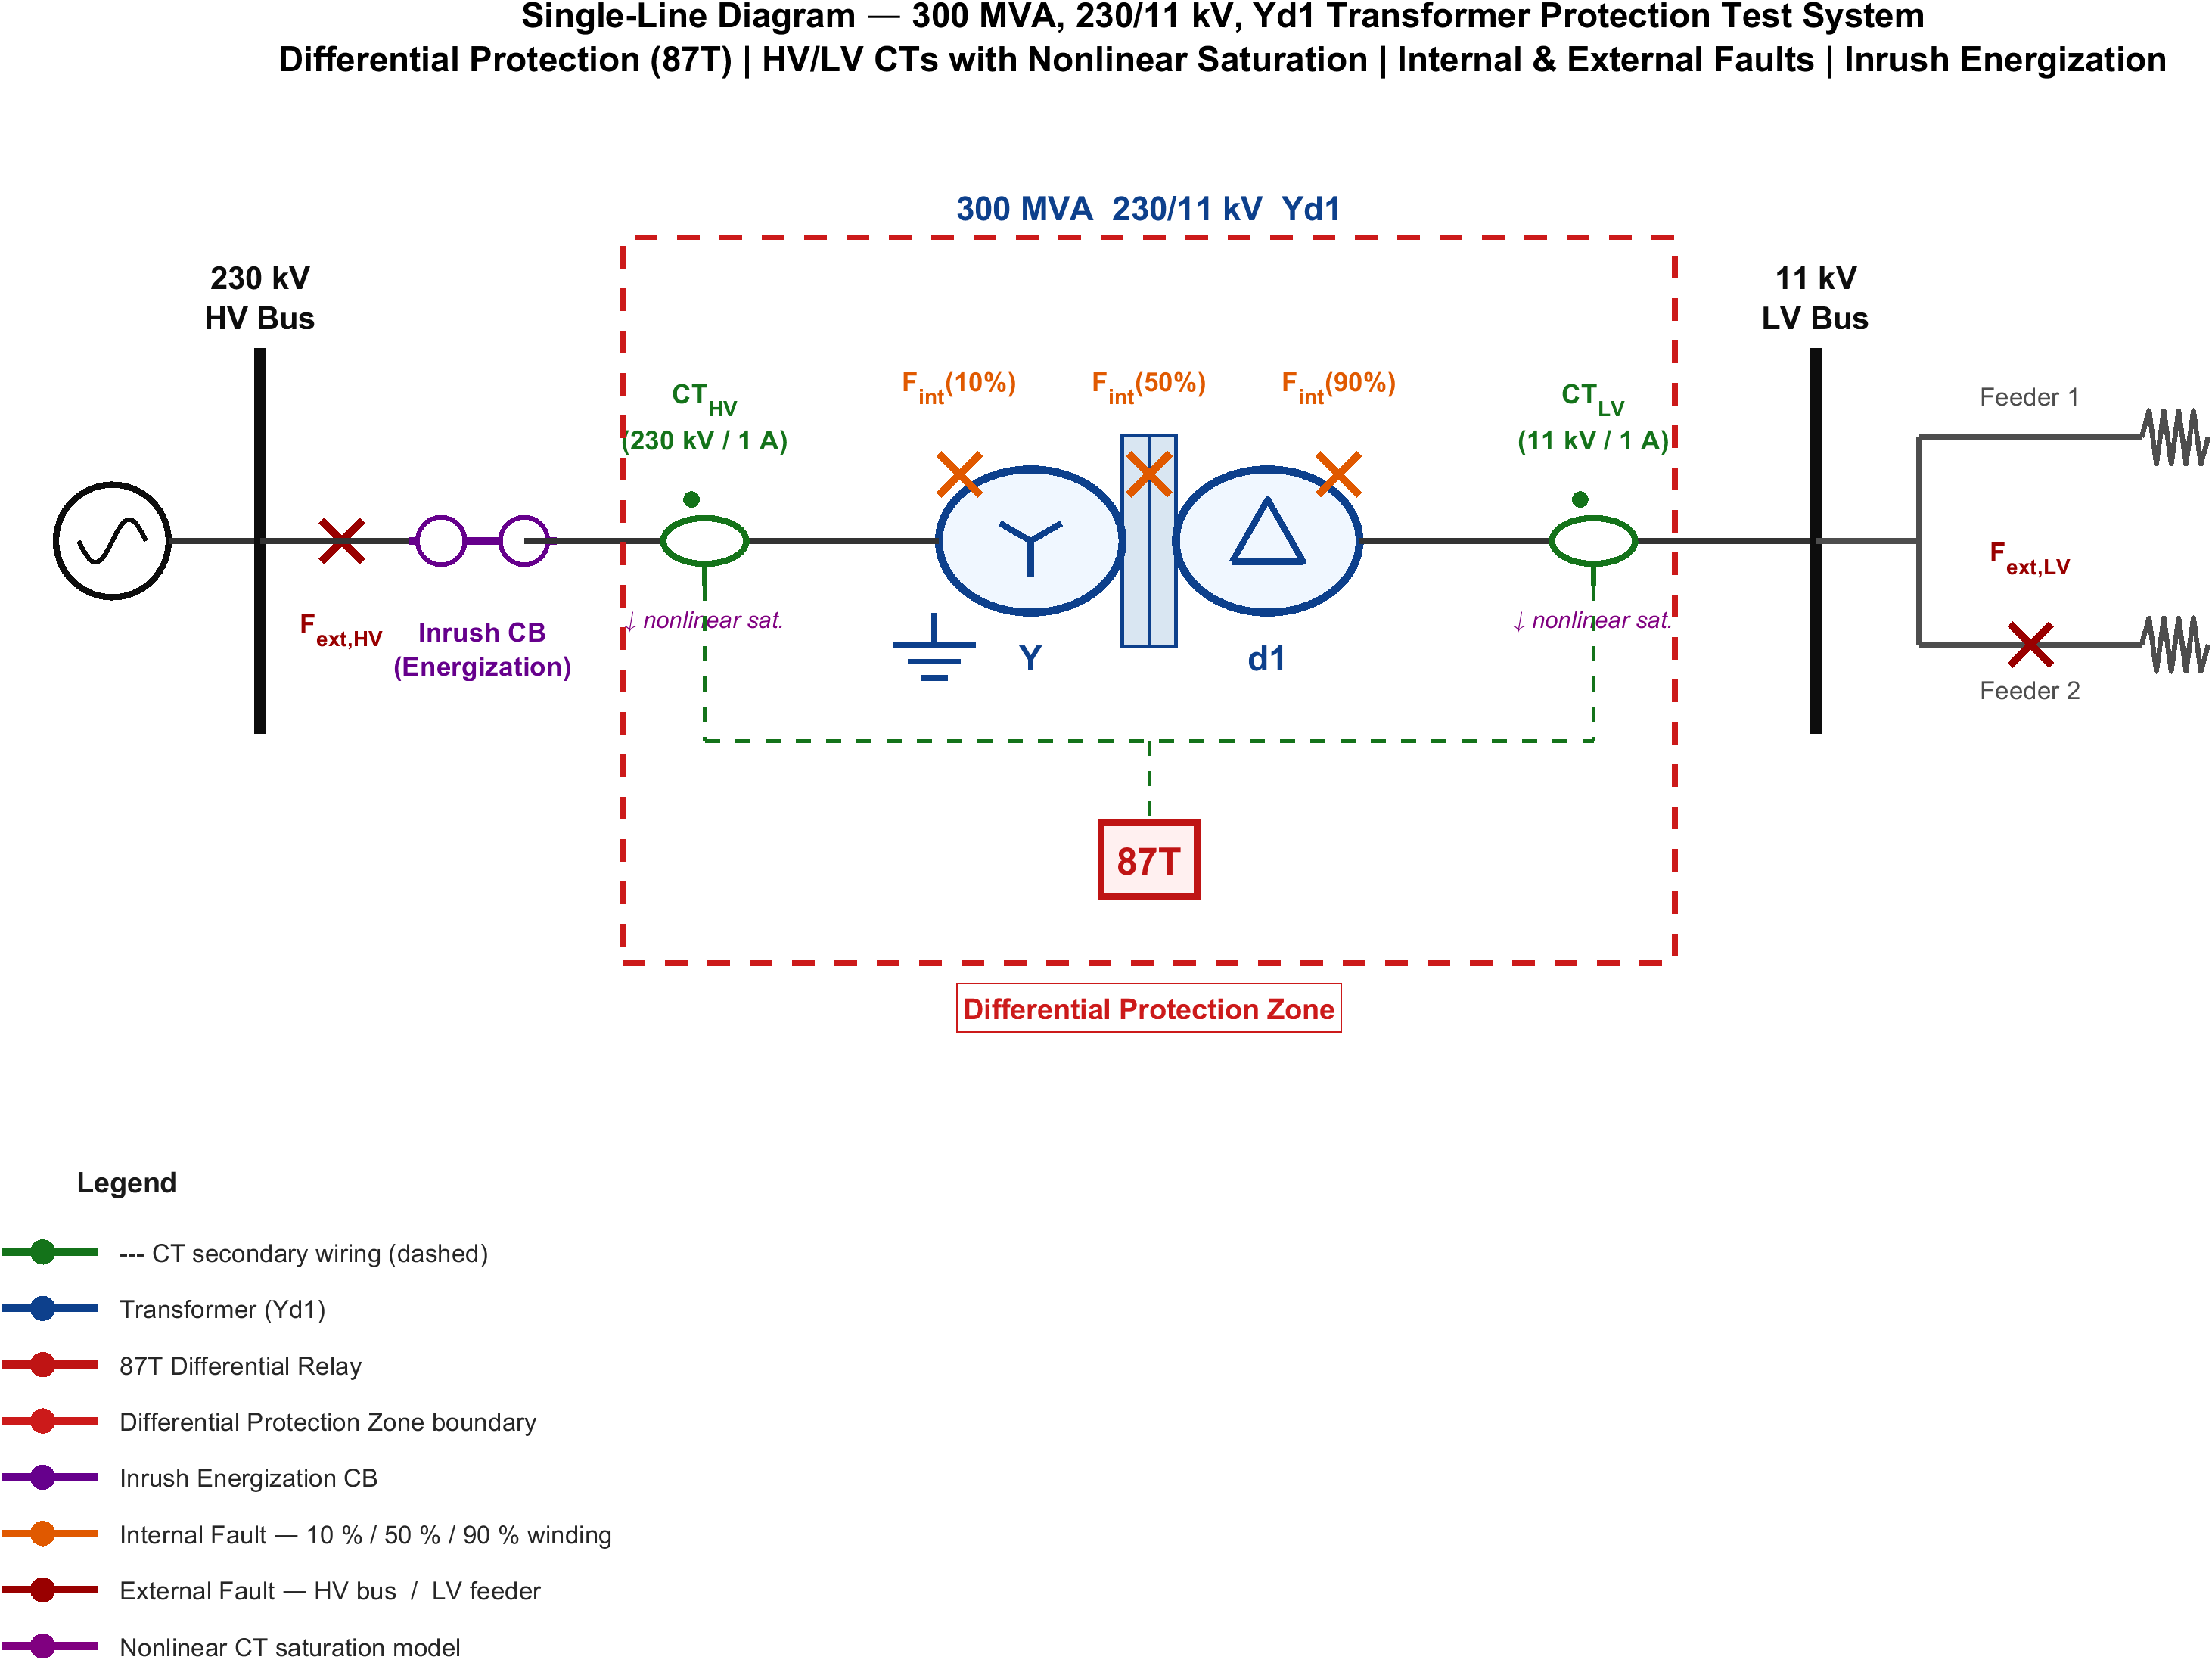
\includegraphics[width=0.75\textwidth]{figures/SLD_300MVA_Yd1_protection.png}
\caption{Single-line schematic of the transformer differential protection zone.}
\label{fig:sld_zone}
\end{figure}
